\documentclass[12pt,a4paper]{report}

\usepackage{styles/dolgozat}

\usepackage{listings}
\usepackage{styles/cpp}
\usepackage{styles/python}

\usepackage{hyperref}

\usepackage{caption}
\usepackage{subcaption}

\begin{document}

\pagestyle{empty}

{\small
Miskolci Egyetem \hfill Miskolci Egyetem

Gépészmérnöki és Informatikai Kar \hfill Gépészmérnöki és Informatikai Kar

Általános Informatikai Intézeti Tanszék \hfill \hfill Alkalmazott Matematikai Intézeti Tanszék}

{\large
\begin{center}
\vglue 1.5truecm

\includegraphics[scale=0.15]{images/me_logo.png}\\
\end{center}}

\vglue 1.5truecm

{\huge
\begin{center}
\textbf{A szakdolgozat címe}
\end{center}}

\vspace*{1cm}

\begin{center}
\LARGE \textbf{Szakdolgozat}
\end{center}

\vspace*{2.5truecm}

{\large
\hspace{6.5cm} \textbf{Készítette}:

%\vskip 2mm

\hspace{6.5cm} \textbf{Név}: Szakdolgozó Neve

%\vskip 1mm

\hspace{6.5cm} \textbf{Neptunkód}: \texttt{NPTNCD}

%\vskip 1mm

\hspace{6.5cm} \textbf{Szak}: Mérnökinformatikus BSc

%\vskip 1mm

\hspace{6.5cm} Korszerű web technológiák szakirány
}

\newpage


\newpage

\pagestyle{empty}

\vspace*{1cm}  
\begin{center}
\large\textsc{\bfseries Eredetiségi Nyilatkozat}
\end{center}
\vspace*{2cm}  

Alulírott \textbf{Szakdolgozó Neve}; Neptun-kód: \texttt{N3P7UN} a Miskolci Egyetem Gépészmérnöki és Informatikai Karának végzős Mérnökinformatikus szakos hallgatója ezennel büntetőjogi és fegyelmi felelősségem tudatában nyilatkozom és aláírásommal igazolom, hogy \textit{Szakdolgozat Címe}
című szakdolgozatom saját, önálló munkám; az abban hivatkozott szakirodalom
felhasználása a forráskezelés szabályai szerint történt.\\

Tudomásul veszem, hogy szakdolgozat esetén plágiumnak számít:
\begin{itemize}
\item szószerinti idézet közlése idézőjel és hivatkozás megjelölése nélkül;
\item tartalmi idézet hivatkozás megjelölése nélkül;
\item más publikált gondolatainak saját gondolatként való feltüntetése.
\end{itemize}

Alulírott kijelentem, hogy a plágium fogalmát megismertem, és tudomásul veszem, hogy
plágium esetén szakdolgozatom visszautasításra kerül.

\vspace*{3cm}

\noindent Miskolc, \hbox to 2cm{\dotfill} .év \hbox to 2cm{\dotfill} .hó \hbox to 2cm{\dotfill} .nap

\vspace*{3cm}

\hspace*{8cm}\begin{tabular}{c}
\hbox to 6cm{\dotfill}\\
Hallgató
\end{tabular}

\newpage


\cleardoublepage
\pagenumbering{gobble}
\tableofcontents
\cleardoublepage
\pagenumbering{arabic}

\newpage

\pagestyle{fancy}

\Chapter{Bevezetés}

Ha nekünk nem is, de nagyszüleinknek bizonyára megtalálhatók még régi, szürkeárnyalatos fényképek a fiók mélyén. Az ilyen régi, családi képeket nézegetve keltette fel az érdeklődésemet a dolgozat témaköre. Érdekelt, hogy vajon hogyan tudnánk az ilyen fotókat életre kelteni színek segítségével.

A képek kiszínezése két problémakörre osztható. 
Az első problémakör azon részek meghatározása a képen, amelyek eredetileg azonos színűek lehettek. Ha mi, emberek ránézünk egy képre, ezt könnyen meg tudjuk határozni, viszont a számítógép számára ez már nem ilyen egyszerű. A dolgozatban több módszert is megvizsgálok annak érdekében, hogy minél pontosabban tudjam meghatározni az azonos színű területeket.

A második problémakör az nem más, mint hogy hogyan tudjuk kiszínezni ezeket az összefüggő részeket, és meghatározni azt a színt, amely a legközelebb állhat az objektum eredeti színéhez. Mint az első problémakörnél, nekünk, embereknek ez szintén nem jelent kihívást, hiszen ha látunk például egy banánt egy szürkeárnyalatos képen, tudjuk, hogy valószínűleg sárga színű lehetett. A számítógépnek viszont meg kell tanítanunk, hogy adott tárgyak, adott textúrák milyen színűek, és ebből megpróbálja kitalálni hogy a szürkeárnyalatos képen szereplő tárgy, textúra milyen színű lehet.

A dolgozat elején bemutatásra kerülnek a probléma megoldásához használt általános eszközök. Azt követően a K-means klaszterező eljárás segítségével láthatjuk, hogy hogyan lehet a képet szegmensekre, régiókra bontani. Ezt a szegmentálás egy érdekes megközelítéseként a szuper pixeles vizsgálatok követik. Végül a képek egyes részeinek színére vonatkozó becslési eljárások következnek.

\Chapter{Koncepció}

\Section{A fejezet célja}

Ez a fejezet még nem a saját eredményekkel foglalkozik, hanem bemutatja, mi a problémakör, milyen módszerekkel, milyen eredményeket sikerült elérni eddig másoknak.

A hivatkozások jelentős része ehhez a fejezethez szokott kötődni.
(Egy hivatkozás például így néz ki \cite{coombs1987markup}.)
Ez szintén egy példa internetes hivatkozásra, a CSS szabvány kapcsán \cite{css}.
Itt lehet bemutatni a hasonló alkalmazásokat.

\Section{Tartalom és felépítés}

A fejezet tartalma témától függően változhat. Az alábbiakat attól függően különböző arányban tartalmazhatják.
\begin{itemize}
\item Irodalomkutatás. Amennyiben a dolgozat egy módszer kidolgozására, kifejlesztésére irányul, akkor itt lehet részletesen végignézni (módszertani vagy időrendi bontásban), hogy az eddigiekben milyen eredmények születtek a témakörben.
\item Technológia. Mivel jellemzően kutatásról vagy szoftverfejlesztésről van szó, ezért annak a jellemző elemeit, technikai részleteit itt kell bemutatni.
Ez tehát egy módszeres bevezetés ahhoz, hogy ha valaki nem jártas a témakörben, akkor tudja, hogy a dolgozat milyen aktuálisan elérhető eredményeket, eszközöket használt fel.
\item Piackutatás. Bizonyos témáknál új termék vagy szolgáltatás kifejlesztése a cél.
Ekkor érdemes annak alaposan utánanézni, hogy aktuálisan milyen eszközök érhetők el a piacon.
Ez szoftverek esetében a hasonló alkalmazások bemutatását, táblázatos formában történő összehasonlítását jelentheti.
Szerepelhetnek képek és észrevételek a viszonyításként bemutatott alkalmazásokhoz.
\item Követelmény specifikáció. Külön szakaszban érdemes részletesen kitérni az elkészítendő alkalmazással kapcsolatos követelményekre.
Ehhez tartozhatnak forgatókönyvek (\textit{scenario}-k).
A szemléletesség kedvéért lehet hozzájuk képernyőkép vázlatokat is készíteni, vagy a használati eseteket más módon szemléltetni.
\end{itemize}

\Section{Amit csak említés szintjén érdemes szerepeltetni}

Az olvasóról annyit feltételezhetünk, hogy programozásban valamilyen szinten járatos, és a matematikai alapfogalmakkal sem ebben a dolgozatban kell megismertetni.
A speciális eszközök, programozási nyelvek, matematikai módszerekk és jelölések persze jó, hogy ha említésre kerülnek, de nem kell nagyon belemenni a közismertnek tekinthető dolgokba.

\Chapter{Általános információk (?)}

Ebben a fejezetben néhány általános információ található, amik a dolgozat teljes egészére érvényesek.

\Section{Felhasznált képek}

A teszteléshez csendéletekről készült képeket gyűjtöttem az unsplash nevezetű weboldalról. \cite{unsplash}
A csendéleteken a tárgyak intenzitása jól elkülönül a háttér intenzitásától így egyszerűbben lehet rajta szegmentálást végrehajtani.
A képek nevei a 0 és 5 közötti számok, pl. 0.jpg.

\Section{Képek feldolgozása}

A képek feldolgozása során előfordulnak olyan lépések, műveletek amelyeket több ponton is megismételtem. Ezeket ebben a bekezdésben szeretném bemutatni, a későbbiekben nem térek ki rájuk részletesen. 
A képfeldolgozáshoz az opencv-python könyvtárat használtam.

\SubSection{Betöltés}

A képeket két módon töltöm be a további feldolgozásra:
\begin{itemize}
\item színesen
\item szürkeárnyalatosan
\end{itemize}
Ehhez két külön metódust készítettem:
\begin{itemize}
\item \texttt{load\_image\_rgb}
\item \texttt{load\_image\_grayscale}
\end{itemize}
Ezek eleinte minden notebookban ismétlődtek, majd a kutatás későbbi szakaszában kiszerveztem őket a \texttt{commonmethods} nevű saját készítésű python librarybe amiről részletesebben a következő alfejezetben írok.

A szürkeárnyalatos kép betöltését a következő kódrészlet tartalmazza.
\begin{python}
import cv2

def load_image_grayscale(name):
    """
    Loading the image from the images folder using opencv-python
    :param name: the name of the image I want to load,
        the method doesn't need the path or the extension
    :return: the loaded image in grayscale color
    """
    image = cv2.imread('../images/' + format(name) + '.jpg')
    image = cv2.cvtColor(image, cv2.COLOR_BGR2GRAY)

    return image
\end{python}
A színes kép betöltése annyiban különbözik, hogy a cv2.COLOR\_BGR2GRAY helyett cv2.COLOR\_BGR2RGB szerepel.

Mind a két metódus a kép nevét várja bemenetként. Mivel a tesztelés során használt képek mindegyike JPG típusú így a kiterjesztést a metódus automatikusan hozzákapcsolja.

\SubSection{Átméretezés}

Átméretezésre a \texttt{resize\_image} metódust készítettem, amelynek a forráskódja a következő:
\begin{python}
import cv2

def resize_image(image, wanted_height) :
    """
    Resizing the image for the given height,
    without disortion, using opencv-python
    :param image: the image that I want to resize
    :param wanted_height: the height in pixel that
        I want to have in the resized image
    :return: the resized image
    """
    height = image.shape[0]
    # calculating the amount with I need to change the width
    scale_percent = height / wanted_height
    width = int(image.shape[0] / scale_percent)
    dim = (width, wanted_height)

    resized_image = \
        cv2.resize(image, dim, interpolation = cv2.INTER_AREA)

    return resized_image
\end{python}
Bemenetként magát a képet várja és azt a méretet px-ben, amire a magasságot szeretnénk változtatni. Hogy ne torzuljon a kép, kiszámítok egy arányt a paraméterként kapott méretből és a kép magasságából, majd ezzel az aránnyal csökkentem a kép szélességét.

\Section{Közös metódusok kiszervezése}

Írni a saját Python libraryről, hogyan kell használni stb. \cite{pythonlibrary}

\Section{Tesztelési környezet}

A programkódok tesztelését minden esetben az otthoni számítógépemen végeztem aminek a paraméterei a következők:
\begin{itemize}
\item Processzor: Intel(R) Core(TM) i5-9400F CPU 2.90GHz
\item Memória mérete: 16 GB
\item (?) Videókártya: NVIDIA GeForce GTX 1660
\item Operációs rendszer: Windows 10 Enterprise
\end{itemize} 
\Chapter{Klaszterezés}

Ahhoz, hogy szürkeárnyalatos képeket megfelelően tudjunk kiszínezni, első lépésként meg kell határoznunk a kiszínezendő területeket. El kell döntenünk hogy a kép mely részei tartoznak ugyan ahhoz a színárnyalathoz és melyek nem. Ezek alapján a dolgozat 2 fő részre bontható:
\begin{itemize}
\item képszegmentálás
\item szegmensek kiszínezése
\end{itemize}

A képszegmentálás célja az, hogy a képen lévő különböző célterületeket elkülönítse, a klaszterezés célja pedig az azonos tulajdonságokkal rendelkező objektumok közös kategóriába sorolása ahol az egy kategóriába tartozó objektumok egymáshoz hasonlóak, viszont különböznek a többi kategóriában lévő objektumoktól.

A két módszer célja lényegében megegyezik egymással. Ahhoz hogy a képből ki tudjuk nyerni a megfelelő szegmenseket, valamilyen klaszterezési eljárást kell alkalmaznunk.

A klaszterezési algoritmusokat a következő módon tudjuk csoportosítani\cite{clustering}:
\begin{itemize}
\item hierarchikus: a korábban létrehozott klaszterek felhasználásával találja meg az egymást követő klasztereket
    \begin{itemize}
    \item agglomeratív (bottom-up): minden egyes elemet különálló klaszterként kezel és azokat nagyobb klaszterekbe egyesíti
    \item osztó (top-down): a teljes halmazból indul ki és azt kisebb klaszterekre osztja
    \end{itemize}
\item particionáló: egyszerre határozza meg az összes klasztert
\item rács alapú: a teret véges számú cellára kvantálja amelyek egy rácsszerkezetet alkotnak, és ezeken hajtja végre a klaszterezést
\item modell alapú: megpróbálja az adatokat optimálisan ráilleszteni valamilyen matematikai modellre
\end{itemize}

A kutatások során az egyik legnépszerűbb particionáló klaszterezést használtam, a k-means klaszterezést.

\Section{K-means klaszterezés}
%TODO dokumentálás
\begin{python}
def kmeans_segmentation(image, k):
    """
    Segmenting the image using opencv-python's k-means method
    :param image: the image that I want to carry out the segmentation
    :param k: the number of the clusters
    :return: the compactness, the pixel_values and the labels
        from the k-means method
    """
    pixel_values = image.reshape((-1, 1))
    pixel_values = np.float32(pixel_values)

    criteria = \
        (cv2.TERM_CRITERIA_EPS + cv2.TERM_CRITERIA_MAX_ITER, 100, 0.2)

    compactness, labels, (centers) = cv2.kmeans(
        pixel_values,
        k,
        None,
        criteria,
        10,
        cv2.KMEANS_RANDOM_CENTERS)

    labels = labels.flatten()

    return compactness, pixel_values, labels
\end{python}

\Section{Optimális klaszterszám meghatározása}

Az optimális klaszterszám meghatározásához 4 módszert teszteltem le, ezeknek az eredménye a következő alfejezetekben található.
A módszereket a \cite{tomatoleaf} és a \cite{elbow} kutatások alapján választottam. 

A módszereknél a klaszterekre bontás idejét nem veszem figyelembe, csak magának a módszernek a futási idejét.

\SubSection{Silhouette módszer}

A Silhouette index azt méri, hogy egy adott objektum mennyire hasonlít a saját klaszterében lévő objektumokhoz. Az értéke +1 és -1 között mozog. A nagyobb érték azt jelzi hogy az objektum jól illeszkedik a saját klaszteréhez és rosszul illeszkedik a szomszédos klaszterekhez. Ha a legtöbb objektumnak pozitív az értéke akkor a klaszterezés megfelelő, ha sok objektumnak negatív, akkor vagy túl sok, vagy túl kevés a klaszter. 

A módszer a következő képlettel írható le:

\[ S(k)=\frac{1}{num} \sum_{i=1}^{num} \frac{b(i)-a(i)}{max\{a(i),b(i)\}} \quad \cite{tomatoleaf} \]

ahol
\begin{itemize}
\item $n$: a klaszterek száma
\item $num$: a pixelek száma
\item $a(i)$: az $i$ minta és az ugyanabban a klaszterben lévő többi minta közötti átlagos távolság
\item $b(i)$: az $i$ minta és az összes többi klaszter mintája közötti távolság minimális értéke
\end{itemize}
Ennek eredményeként megkapjuk a Silhouette pontszámot. Ha elvégezzük ezt a vizsgálatot különböző klaszterszámokra, akkor amelyiknek a pontszáma a legnagyobb, az lesz a legoptimálisabb klaszterszám. 

Vizsgálataim során a \texttt{sklearn.metrics} csomagban található \texttt{silhouette\_score} módszert használtam a következő kódrészletben látható módon. Ez a metódus megtalálható az általam készített \texttt{commonmethods} csomagban.
\begin{python}
def silhouette_method(values, labels):
    """
    Calculating the Silhouette method for the given values with
    the given labels, and measuring time.
    :param values: in my case the pixel values from the k-means method
    :param labels: in my case the labels from the k-means method
    :return: the time of the calculation and
        the calculated Silhouette score
    """
    start = time.time()
    s_score = silhouette_score(values, labels)
    end = time.time()

    s_time = end-start

    return s_time, s_score
\end{python}
Mint látható, a metódus visszatér a módszer számítási idejével, mivel a vizsgálataim során a futási idők összevetése volt az egyik fő szempont. Ezen kívül visszaadja a kiszámított Silhouette pontszámot is, amit az általam megadott értékekből és a hozzájuk tartozó címkékből állít elő. Ezeket az értékeket a \texttt{kmeans\_segmentation} metódus eredményeként kapom.

A Silhouette módszer esetén azt tapasztaltam, hogy a futási ideje elég lassú. A \ref{fig:silhouette_runtime} ábrán látható a módszer futási ideje különböző méretű képekre.

\begin{figure}[h]
\centering
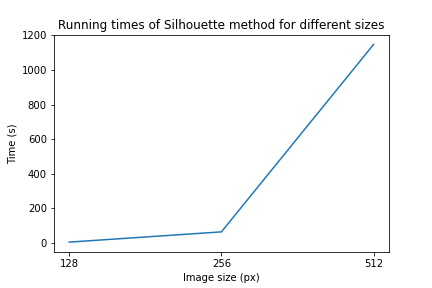
\includegraphics[scale=0.9]{images/silhouette_runtime.png}
\caption{A Silhouette módszer futási ideje különböző képméretekre.}
\label{fig:silhouette_runtime}
\end{figure}

Jól látható, hogy míg a 128px méretű képre pár másodperc alatt elvégzi a számítást, az 512px méretű képre már nagyságrendileg 20 percig számol.

\SubSection{Davies-Bouldin módszer}
A Davies-Bouldin index a klaszteren belüli szóródás összegének és a klaszterek közötti szétválás arányának a függvénye. A célunk az, hogy ezt az értéket minimalizáljuk, hiszen azt szeretnénk hogy a klaszteren belüli szórás minimális, a klaszterek közötti elkülönülés pedig maximális legyen.

A módszer képlete a következő:

\[ DB(k)=\frac{1}{k} \sum_{i=1}^{K} max \left(\frac{W_i + W_j}{C_{ij}}\right)  \quad \cite{tomatoleaf} \]

ahol
\begin{itemize}
\item $K$: a klaszterek száma
\item $W_i$: a $C_i$ osztályba tartozó összes minta átlagos távolsága a klaszter középpontjától
\item $W_{j}$: a $C_i$ osztályba tartozó összes minta átlagos távolsága a $C_j$ osztály középpontjától 
\item $C_{ij}$: a $C_i$ és $C_j$ osztályok középpontja közötti távolság
\end{itemize}
Ennek eredményeként megkapjuk a Davies-Bouldin pontszámot. Ha elvégezzük ezt a vizsgálatot különböző klaszterszámokra, akkor amelyiknek a pontszáma a legkisebb, az lesz a legoptimálisabb klaszterszám.

Ennek a módszernek a megvalósításához a \texttt{sklearn.metrics} csomagban található \texttt{davies\_bouldin\_score} metódust használtam. A következő kódrészletben látható, hogy a módszer megvalósítása ugyan arra a sémára épül, mint a \texttt{silhouette\_method}. 

Ez a metódus is megtalálható az általam készített \texttt{commonmethods} csomagban.
\begin{python}
def davies_bouldin_method(values, labels):
    """
    Calculating the Davies-Bouldin method for the given values with
    the given labels, and measuring time.
    :param values: in my case the pixel values from the k-means method
    :param labels: in my case the labels from the k-means method
    :return: the time of the calculation and
        the calculated Davies-Bouldin score
    """
    start = time.time()
    db_score = davies_bouldin_score(values, labels)
    end = time.time()

    db_time = end-start

    return db_time, db_score
\end{python}

\SubSection{Calinski-Harabasz módszer}

A Calinski-Harabasz indexet belső klaszterérvényességi mérőszámként szokták használni, amely a létrehozott klasztereket osztályozza.

A módszer képlete a következő \cite{silhouette_calinski}:

\begin{equation*}
\begin{split} \label{}
 CH(k) & =\frac{B(K)(N-K)}{W(K)(K-1)} \\
 & B(K)=\sum_{k=1}^{K}a_k \|\overline{x_k}-\overline{x}\|^2 \\
 & W(K)=\sum_{k=1}^{K}\sum_{C(j)=k}\|x_j-\overline{x_k}\|^2
\end{split}
\end{equation*}

ahol
\begin{itemize}
\item $K$: a klaszterek száma
\item $N$: a minta száma
\item $B(K)$: a klaszterek közötti divergencia, más néven a klaszterek közötti kovariancia
\item $W(K)$: a klaszteren belüli divergencia, más néven a klaszteren belüli kovariancia
\end{itemize}

Minél nagyobb a $B(K)$ értéke, annál nagyobb a klaszterek közötti diszperzió mértéke. Minél kisebb a $W(K)$ értéke, annál szorosabb a kapcsolat a klaszteren belül. Minél nagyobb az arány, annál nagyobb a Calinski-Harabasz pontszám értéke, theát annál optimálisabb a klaszterszám.

Ennek a módszernek a megvalósításához a \texttt{sklearn.metrics} csomagban található \texttt{calinski\_harabasz\_score} metódust használtam. A következő kódrészletben látható hogy, a módszer megvalósítása ugyan arra a sémára épül, mint a \texttt{silhouette\_method} és a \texttt{davies\_bouldin\_method}. 

Ez a metódus is megtalálható az általam készített \texttt{commonmethods} csomagban.
\begin{python}
def calinski_harabasz_method(values, labels):
    """
    Calculating the Calinski-Harabasz method for the given values with
    the given labels, and measuring time.
    :param values: in my case the pixel values from the k-means method
    :param labels: in my case the labels from the k-means method
    :return: the time of the calculation and
        the calculated Calinski-Harabasz score
    """
    start = time.time()
    ch_score = calinski_harabasz_score(values, labels)
    end = time.time()

    ch_time = end-start
\end{python}

\SubSection{Elbow módszer}

Az Elbow módszer a variancia százalékos arányát vizsgálja a klaszterek számának függvényében. Azon az elven alapszik hogy olyan klaszterszámot kell választanunk, amelyhez ha hozzáadnánk akár csak egy klasztert is, akkor a modellünk már nem javulna számottevő mértékben. 

Az első klaszterek sok információt adnak hozzá a modellhez, viszont egy bizonyos ponton a határnyereség drámaian lecsökken és szöget, vagyis könyököt képez a grafikonon lásd. \ref{fig:elbow_example}. ábra. Innen ered az "elbow" azaz "könyök" módszer elnevezés. Az a pont ahol ez a drámai csökkenés bekövetkezik, az lesz a megfelelő klaszterszám. A \ref{fig:elbow_example}. ábrán ez a pont 2 klaszternél alakul ki, de érdemes lehet megvizsgálni a 3 klasztert is. \cite{elbow}

\begin{figure}[h]
\centering
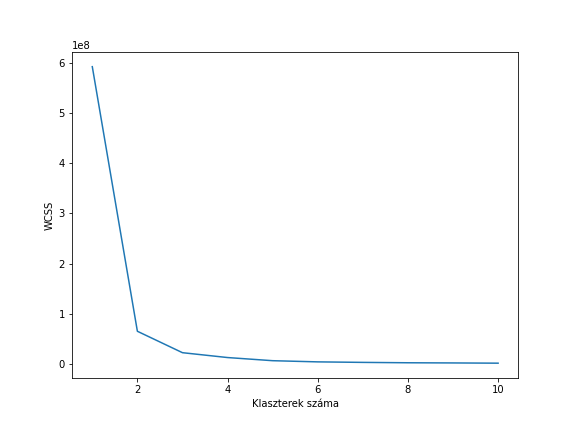
\includegraphics[scale=0.9]{images/elbow_example.png}
\caption{Példa az Elbow módszerre.}
\label{fig:elbow_example}
\end{figure}

Az Elbow metódushoz a \texttt{kmeans\_segmentation} által eredményként visszaadott \texttt{compactness} értékeket szükséges lementenünk különböző méretű klaszterekre ahogy az a következő kódrészletben látható.
\begin{python}
import commonmethods.image_modification as im

wcss = []   #within cluster sum of squares

for i in range(1, 11):
    compactness, pixel_values, labels = \
        im.kmeans_segmentation(resized_image, i)
    wcss.append(compactness)
\end{python}

Ezek után a \texttt{wcss} listát \texttt{plot} segítségével ábrázoljuk és meg is kaptuk az Elbow grafikonunkat, pont úgy mint ahogy a \ref{fig:elbow_example}. ábrán szerepel.

Ennél a módszernél külön számítást nem kell végeznünk, így futási ideje igazából csak maga a kirajzolás.

Összességében a módszer gyors, viszont nem mindig ad egyértelmű eredményt és a töréspont automatizált meghatározása sem egy egyszerű feladat. Vizuális ábrázolásra és kézi ellenőrzésre viszont megfelelő, így főként én is erre a célra használtam.

\SubSection{Összegzés}

A módszerek vizsgálata során hamar kiderült, hogy a Silhouette módszer futási ideje számottevően nagyobb a többi módszerétől. Az eredmények összehasonlítását a \ref{tab:size_runtimes}. táblázat tartalmazza. Mivel az Elbow módszer nem egyértelmű és főként vizuális megerősítésként szolgál, így azt a módszert kihagytam a további elemzésekből.

\begin{table}[h]
\centering
\caption{Futási idők átlaga különböző módszerek esetén}
\label{tab:size_runtimes}
\medskip
\begin{tabular}{|l|c|c|c|c|}
\cline{2-5}
 \multicolumn{1}{c|}{} & \multicolumn{4}{c|}{Kép mérete} \\
 \hline
 Módszer & 64px & 128px & 256px & 512px \\
\hline
Silhouette módszer & 0.2684s & 4.4029s & 68.0697s & 1183.2937s \\
Davies-Bouldin módszer & 0.0071s & 0.0042s & 0.0096s & 0.0274s \\
Calinski-Harabasz módszer & 0.0031s & 0.001s & 0.0028s & 0.0120s \\
\hline
\end{tabular}
\end{table}

Mivel a klaszterek számának növelésével a feldolgozandó adathalmaz nem változik így a klaszterek száma nem befolyásolja a módszerek futási idejét. Erre bizonyítékként szolgál a \aref{tab:cluster_runtimes}. táblázat amely különböző klaszterszám esetén mutatja be az átlagos futási időket. Jól látható hogy nem növekszik, sőt valahol csökken a magasabb klaszterszám esetén a futási idő.

\begin{table}[h]
\centering
\caption{Futási idők átlaga különböző klaszterszámok és módszerek esetén, 256px képméretre}
\label{tab:cluster_runtimes}
\medskip
\begin{tabular}{|l|c|c|c|}
\cline{2-4}
 \multicolumn{1}{c|}{} & \multicolumn{3}{c|}{Klaszterek száma} \\
 \hline
 Módszer & 2 & 4 & 8 \\
\hline
Silhouette módszer & 63.1462s & 63.1254s & 62.2278s \\
Davies-Bouldin módszer & 0.0060s & 0.0083s & 0.0064s \\
Calinski-Harabasz módszer & 0.0026s & 0.0024s & 0.0028s \\
\hline
\end{tabular}
\end{table}

Természetesen a k-means metódus lassabban határozza meg a klasztereket nagyobb klaszterszám esetén így a nagyobb klaszterszám magának a programnak a futási idejét befolyásolja. 

%TODO Jósági vizsgálat és dokumentálása
\Chapter{Megvalósítás}

Ez a fejezet mutatja be a megvalósítás lépéseit.
Itt lehet az esetlegesen előforduló technikai nehézségeket említeni.
Be lehet már mutatni a program elkészült részeit.

Meg lehet mutatni az elkészített programkód érdekesebb részeit.
(Az érdekesebb részek bemutatására kellene szorítkozni.
Többségében a szöveges leírásnak kellene benne lennie.
Abból lehet kiindulni, hogy a forráskód a dolgozathoz elérhető, azt nem kell magába a dolgozatba bemásolni, elegendő csak behivatkozni.)

A dolgozatban szereplő forráskódrészletekhez külön vannak programnyelvenként stílusok.
Python esetében például így néz ki egy formázott kódrészlet.
\begin{python}
import sys

if __name__ == '__main__':
    pass
\end{python}

A stílusfájlok a \texttt{styles} jegyzékben találhatók.
A stílusok között szerepel még C++, Java és Rust stílusfájl.
Ezek használatához a \texttt{dolgozat.tex} fájl elején \texttt{usepackage} paranccsal hozzá kell adni a stílust, majd a stílusfájl nevével megegyező környezetet lehet használni.
További példaként C++ forráskód esetében ez így szerepel.
\begin{cpp}
#include <iostream>

class Sample : public Object
{
    // An empty class definition
}
\end{cpp}
Stílusfájlokból elegendő csak annyit meghagyni, amennyire a dolgozatban szükség van.
Más, C szintaktikájú nyelvekhez (mint például a JavaScript és C\#) a Java vagy C++ stílusfájlok átszerkesztésére van szükség.
(Elegendő lehet csak a fájlnevet átírni, és a fájlban a környezet nevét.)

Nyers adatok, parancssori kimenetek megjelenítéséhez a \texttt{verbatim} környezetet lehet használni.
\begin{verbatim}
$ some commands with arguments
1 2 3 4 5
$ _
\end{verbatim}

A kutatás jellegű témáknál ez a fejezet gyakorlatilag kimaradhat.
Helyette inkább a fő vizsgálati módszerek, kutatási irányok kaphatnak külön-külön fejezeteket.

\Chapter{Tesztelés}

A fejezetben be kell mutatni, hogy az elkészült alkalmazás hogyan használható.
(Az, hogy hogyan kell, hogy működjön, és hogy hogy lett elkészítve, az előző fejezetekben már megtörtént.)

Jellemzően az alábbi dolgok kerülhetnek ide.
\begin{itemize}
\item Tesztfuttatások. Le lehet írni a futási időket, memória és tárigényt.
\item Felhasználói kézikönyv jellegű leírás. Kifejezetten a végfelhasználó szempontjából lehet azt bemutatni, hogy mit hogy lehet majd használni.
\item Kutatás kapcsán ide főként táblázatok, görbék és egyéb részletes összesítések kerülhetnek.
\end{itemize}

\Chapter{Összegzés}

Hasonló szerepe van, mint a bevezetésnek.
Itt már múltidőben lehet beszélni.
A szerző saját meglátása szerint kell összegezni és értékelni a dolgozat fontosabb eredményeit.
Meg lehet benne említeni, hogy mi az ami jobban, mi az ami kevésbé jobban sikerült a tervezettnél.
El lehet benne mondani, hogy milyen további tervek, fejlesztési lehetőségek vannak még a témával kapcsolatban.

\Chapter{Summary}

The content of the previous chapter in english.

\clearpage

\addcontentsline{toc}{chapter}{Irodalomjegyzék}
\bibliographystyle{unsrt}
\bibliography{dolgozat}

\noindent \textit{Az internetes források utolsó ellenőrzése: 2021.10.05}

\pagestyle{empty}

\newpage

\pagestyle{empty}

\noindent \textbf{\Large CD melléklet tartalma}

\vskip 1cm

\noindent A dolgozathoz mellékelt lemezen egy \texttt{Dolgozat} nevű jegyzékben a következő fájlok találhatóak.

\begin{itemize}
\item A dolgozat \LaTeX\ forráskódja.
\item A dolgozat PDF formátumban (\texttt{dolgozat.pdf}).
\item A magyar és angol nyelvű összefoglaló \LaTeX\ és PDF formátumban \\ (\texttt{osszegzes.tex}, \texttt{osszegzes.pdf}, \texttt{summary.tex}, \texttt{summary.pdf}).
\end{itemize}

Az \texttt{images} nevű jegyzékben találhatóak a vizsgálatokhoz használt mintaképek.

A \texttt{notebooks} jegyzékbe kerültek a dolgozat megírása során elkészített és az abban részletezett Jupyter munkafüzetek.

A \texttt{program} nevű jegyzékben található a dolgozathoz Python szkriptekként elkészített programok.


\end{document}
